% calculus:x02
\begin{question}
  \hspace*{\fill} [Note maximale: 15]\par
  \noindent Une boîte en métal, cylindrique et fermée, de rayon égal à $r$ centimètres et de hauteur égale à $h$ centimètres possède un volume de $20\pi$ $cm^3$.\par
  
  \medskip
  \begin{flushleft}
    \noindent La figure n'est pas a l'échelle\par
    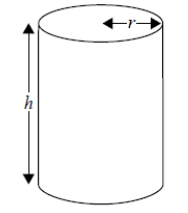
\includegraphics[scale=0.5]{cylindre.png}\par
  \end{flushleft}
  \medskip

  (a) Exprimez $h$ en fonction de $r$.\hspace*{\fill} [2]\par
  \medskip
  \noindent Le métal pour la base et le couvercle de la boîte coûte 10 cents le $cm^2$ et le métal pour le côté incurvé coûte 8 cents le $cm^2$. Le coût total du métal, en cents, est de $C$.\par
  \medskip
  (b) Montrez que $C$ $=$ $20\pi{}r^2 + \frac{320\pi}{r}$\hspace*{\fill} [4]\par
  \medskip

  (c) Sachant qu’il existe une valeur minimale pour $C$, trouvez cette valeur minimale en fonction de $\pi$ \hspace*{\fill} [9]\par
\end{question}

